\chapter{Διάλογος και Συστάσεις}

Σε αυτό το κεφάλαιο θα περιγράψουμε πολύ περιληπτικά την χρήση της ενισχυτικής μάθησης σε διαλογικά συστήματα, ώστε να μπορέσουμε να το συνδέσουμε με το πρόβλημα μας, και μετά θα περιγράψουμε την χρήση ενισχυτικής μάθησης σε προβλήματα συστάσεων, που είναι και πιο κοντά στο πεδίο του προβλήματος μας.

\section{Διάλογικά Συστήματα}

Η ιδέα της δημιουργίας ενός πράκτορα που θα μπορεί να απαντήσει σε ανθρώπινες ερωτήσεις, ξεκίνησε από το σύγγραμα του \en{Alan Turing, Computing Machinery and Intelligence} \cite{turing1950computing}. Τα πρώτα μοντέλα που δημιουργήθηκαν βασίζονταν σε κανόνες, όπου αναγνώριζαν κάποιες λέξεις-κλειδία στο κείμενο και ανάλογα με αυτές απαντούσαν στον χρήστη. Το πρόβλημα αυτών των συστημάτων ήταν ότι ήταν πολύ δύσκολο να επεκταθούν, καθώς και να γενικεύσουν, αφού η δημιουργοί πρέπει να προσθέσουν χειροκίνητα τους επιπλέον κανόνες. Τα τελευταία χρόνια, η δημιουργία διαλογικών συστημάτων γίνεται ολοένα και περισσότερο με χρήση βαθειάς μηχανικής μάθησης, παρόλο που η χρήση κανόνων είναι ακόμα βολική σε κάποιες περιπτώσεις.

Tα διαλογικά συστήματα συνήθως χωρίζονται σε δύο κατηγορίες ανάλογα με τον σκοπό τους:
\begin{enumerate}
    \item Συγκεκριμένου σκοπού (\en{task-oriented systems}). Τα διαλογικά αυτά συστήματα έχουν ως στόχο να βοηθήσουν τον χρήστη να πετύχει συγκεκριμένους στόχους, ιδανικά σε όσο λιγότερους γύρους διαλόγου γίνεται. Για παράδειγμα τέτοια συστήματα είναι συστήματα μέσω των οποίων ο χρήστης μπορεί να κλείσει εισητήρια, ή να λάβει υποστήριξη σχετικά με ένα πρόβλημα του.
    \item Ανοιχτού σκοπού (\en{open-domain systems}). Τα διαλογικά συστήματα αυτά δεν έχουν κάποιο σκοπό, αλλά εστιάζουν στο να δώσουν ρεαλιστικές απαντήσεις σε συζητήσεις με τον χρήστη.
\end{enumerate}

\begin{figure}
    \centering
    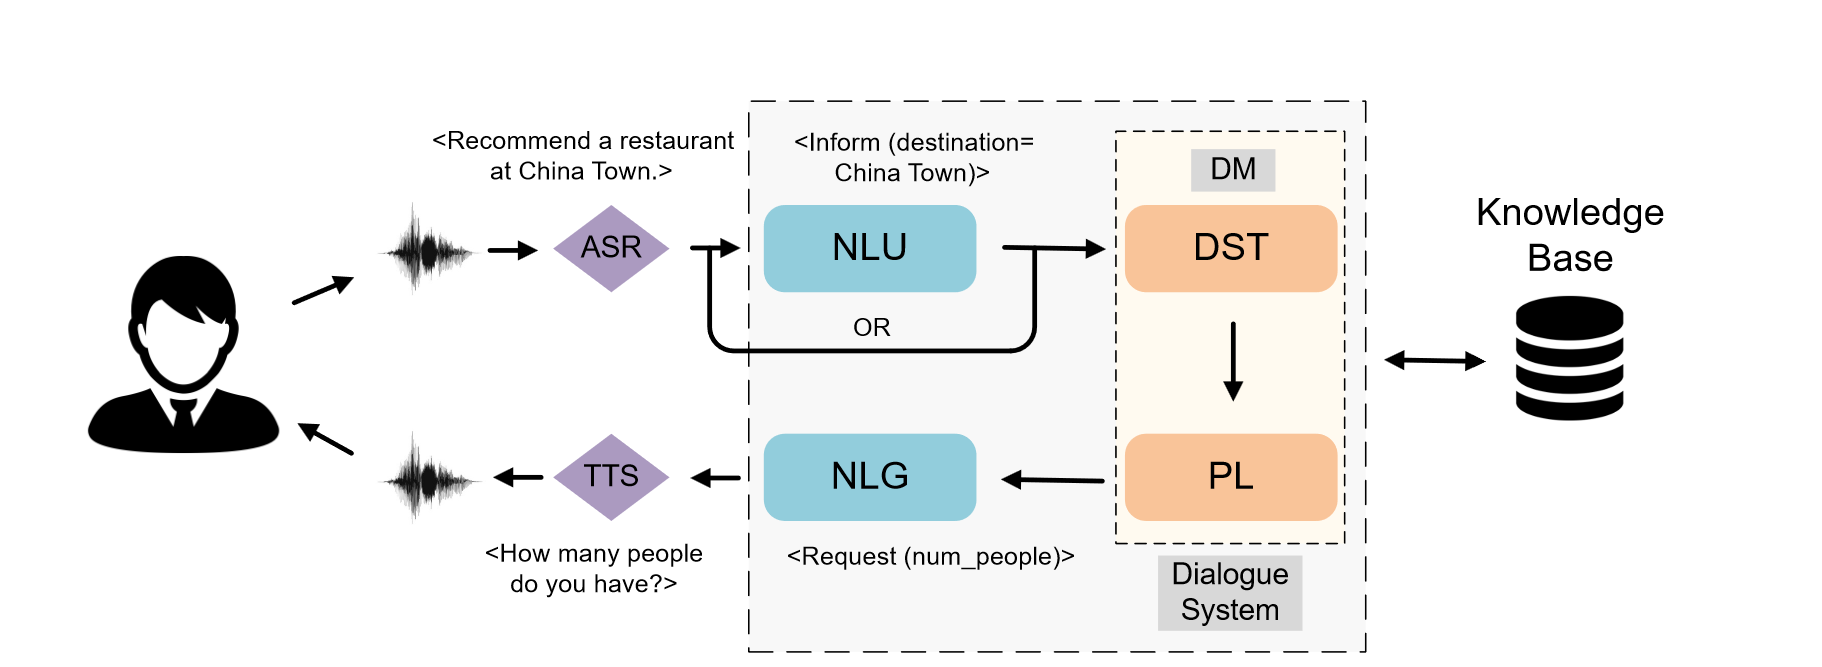
\includegraphics[width=\textwidth]{body_matter/dialogue_and_recommendations/images/task-based-dialogue-system.png}
    \caption{Σύστημα συγκεκριμένου σκοπού \cite{recent_advances_dl_2021}}
    \label{fig:task_based_system}
\end{figure}

Συχνά τα συστήματα συγκεκριμένου σκοπού οργανώνονται σε μια αλληλουχία μερών όπως αυτή που φαίνεται στο Σχήμα~\ref{fig:task_based_system}:
\begin{itemize}
    \item \textbf{Το κομμάτι της κατανόησης της εισόδου του χρήστη.} Αυτό το κομμάτι είνα υπευθυνο για την ταξινόμηση των διάφορων λέξεων σε μέρη του λόγου, την αναγνώριση ονομάτων, αλλά και την αναγνώριση της πρόθεσης του χρήστη με βάση το τι είπε. Κάποια συστήματα δεν χρησιμοποιούν αυτό το κομμάτι και χρησιμοποιούν το ίδιο το μήνυμα του χρήστη ως είσοδο στο επόμενο κομμάτι, όπως στο Σχήμα~\ref{fig:task_based_system}. Αυτό συμβαίνει για να μειώσουν την επίδραση του λάθους του πρώτου αυτού του κομματιού και την μεταφορά λαθών στα μετέπειτα κομμάτια.
    \item \textbf{Το κομμάτι της διαχείρισης της κατάστασης του διαλόγου,} το οποίο ρυθμίζει τις καταστάσεις του διαλόγου με βάση την τρέχουσα είσοδο και την ιστορία του διαλόγου. Η κατάσταση του διαλόγου περιέχει σχετικές δράσεις του χρήστη και ζευγάρια θέσης-τιμής.
    \item \textbf{Το κομμάτι της εκμάθησης της πολιτικής του διαλόγου}, το οποίο με βάση τις καταστάσεις του διαλόγου που παίρνει από το προηγούμενο κομμάτι, επιλέγει την επόμενη δράση του διαλογικού πράκτορα.
    \item \textbf{Το κομμάτι της παραγωγής της απάντησης του συστήματος}, το οποίο μετατρέπει τις δράσεις που επιλέχθηκαν από το προηγούμενο κομμάτι σε φυσική γλώσσα, η οποία θα επιστραφεί στον χρήστη.
\end{itemize}

Άλλες φορές προτιμάται ένα σύστημα που υλοποιεί όλες τις παραπάνω λειτουργίες από άκρη σε άκρη, το οποίο μπορεί να πετύχει καλύτερη βελτιστοποίηση, καθώς δεν υπάρχει μεταφορά σφάλματος μεταξύ των διάφορων κομματιών.

\subsection{Ενισχυτική Μάθηση και Διαλογικά Συστήματα}

Όσον αφορά την χρήση ενισχυτικής μάθησης, σε συστήματα συγκεκριμένου σκοπού είναι στην διαχείρηση του διαλόγου. Πιο συγκεκριμένα δύο σύνηθεις χρήσεις είναι για την παρακολούθηση της κατάστασης του διαλόγου και την εκμάθηση της πολιτικής. Η δεύτερη χρήση είναι ιδιαίτερα σύνηθης και αρκετά επιτυχημένη, καθώς περιγράφεται ακριβώς από ένα πρόβλημα ΕΜ (πχ \cite{policy_learning_2019}).

Σε συστήματα ανοιχτού σκοπού, η χρήση της ενισχυτικής μάθησης είναι κυρίως η επιλογή απαντήσεων παρά η παραγωγή τους, καθώς τα παραγωγικά \en{generative} συστήματα είναι πολύ καλύτερα στην παραγωγή λόγου.

Για παράδειγμα, σε μια από τις πρώτες δουλείες οι οποίες χρησιμοποιήσαν ΕΜ σε διάλογο \cite{rl_dialogue_2016}, οι συγγραφείς προσπάθησαν να ενώσουν τις ιδέες από τα \en{seq2seq} μοντέλα και την ΕΜ, ώστε να δημιουργήσουν συστήματα τα οποία επιστρέφουν καλύτερες απαντήσεις. Έτσι δημιούργησαν μια μετρική ανταμοιβής η οποία αξιολογούσε την ποιότητα των απαντήσεων. Αρχικά εκπαίδευσαν ένα \en{seq2seq} μοντέλο με επιβλεπόμενη μάθεση, και μετά με βάση αυτό προσομοιώσαν διαλόγους μεταξύ δυο πρακτόρων, ξεκινώντας από μια πρόταση από το σύνολο εκπαίδευσης.

Ενα από τα πιο διάσημα σύχρονα παραδείγματα είναι η χρήση του στην εκπαίδευση του \en{InstructGPT}. Στο \cite{chatgpt_2022}, οι ερευνητές έκαναν \en{fine-tune} το {GPT-3} με χρήση ενισχυτικής μάθησης και ανατροφοδότησης από ανθρώπους. Συγκεκριμένα, κατα το \en{fine-tuning}, το μοντέλο "ρώταγε" τους χρήστες ποιά από τις απαντήσεις θεωρούσαν καλύτερη σε σχέση με ένα ερώτημα, οι χρήστες ταξινομούσαν τις απαντήσεις από καλύτερη προς χειρότερη, και με βάση αυτό εκπαιδεύτηκε ένα μοντέλο ανταμοιβών. Έπειτα, για την εκπαίδευση της πολιτικής των απαντήσεων του συστήματος, ενα ερώτημα επιλεγόταν από το σύνολο των δεδομένων, η πολιτική του συστήματος παράγει μια έξοδο και το μοντέλο ανταμοιβών επιλέγει την ανταμοιβή για αυτή την έξοδο. Με βάση αυτό ανανεώνεται η ανταμοιβή της πολιτικής.

\section{Συστήματα Συστάσεων}

Στην πραγματική ζωή, υπάρχουν πολλές περιπτώσεις που πρέπει να πάρουμε μια απόφαση, χωρίς να έχουμε κάποια προηγούμενη πληροφορία σχετικά με την κάθε επιλογή. Έτσι πολλές φορές βασιζόμαστε σε συστάσεις από άλλους, οι οποίοι έχουν παραπάνω εμπειρία στο θέμα, να μας βοηθήσουν.Έτσι δημιουργήθηκε το πρώτο αυτοματοποιημένο σύστημα με αυτό το σκοπό, το οποίο πήρε το όνομα \textit{συνεργατικό φιλτράρισμα} (\en{collaborative filtering}). Αργότερα δημιουργήθηκε ο γενικότερος όρος \textit{σύστημα συστάσεων} για να αναδείξει δύο γεγονότα: 1) Η μέθοδος δεν χρειάζεται να βασίζεται σε αφανή συνεργασία μεταξύ των χρηστών, 2) η μέθοδος μπορεί να προτείνει ενδιαφέροντα αντικείμενα, και όχι να τα φιλτράρει.

Ένα σύστημα συστάσεων αποτελείται από εργαλεία και αλγορίθμους οι οποίοι αναπτύχθηκαν με την ιδέα να βοηθήσουν τους χρήστες να βρουν αντικείμενα που τους ενδιαφέρουν. Σε μια γενική μορφή, ο στόχος είναι η δημιουργία του προφίλ των χρηστών βασισμένη στην ανατροφοδότηση μεταξύ συστήματος και χρήστη και η σύσταση αντικειμένων που να ταιριάζουν στο προφίλ αυτό. Το πρόβλημα απαντάται σε πολλούς κλάδους όπως της υγείας, της διασκέδασης, της ενημέρωσης, κλπ.

Παραδοσιακά το πρόβλημα των συστάσεων θεωρούνταν ένα πρόβλημα ταξινόμησης ή πρόβλεψης, αλλά πλεον η ακαδημαϊκή κοινότητα συμφωνεί ότι η αλληλεπίδραση μεταξύ χρήστη και συστήματος μοντελοποιειται καλύτερα ως ενα πρόβλημα αποφάσεων με διαδοχικά βήματα \cite{rl_recommenders_2021}. Έτσι μπορεί να περιγραφεί από μια Μαρκοβιανή Διαδικασία Αποφάσεων και να λυθεί με χρήση ενισχυτικής μάθησης.

Πριν περάσουμε σε τεχνικές με χρήση ενισχυτικής μάθησης, είναι σημαντικό να γνωρίσουμε περιληπτικά τους κλασικούς αλγορίθμους. Αυτοί είναι:
\begin{itemize}
    \item \textit{Συνεργατικό φιλτράρισμα}: Η ιδέα της μεθόδου είναι η ομαδοποίηση του χρήστη (ή των αντικειμένων) σε ομάδες με παρόμοια χαρακτηριστικά. Όταν το φιλτράρισμα γίνεται με βάση τον χρήστη, οι προτάσεις γίνονται με βάση τις παρόμοιες προτιμήσεις διάφορων χρηστών. Από την άλλη, όταν αναφερόμαστε σε φιλτράρισμα με βάση τα αντικείμενα, οι προτάσεις γίνονται με βάση τα αντικείμενα τα οποία σχετίζονται με αυτά που ο χρήστης έχει ήδη αλληλεπιδράσει. Η μέθοδος αυτή μπορεί να χωριστεί σε δύο προσεγγίσεις: με βάση την μνήμη, όπου ουσιαστικά για κάθε χρήστη/αντικείμενο γίνεται μια σύγκριση ομοιότητας (πχ ομοιότητα συνημιτόνου) με τους υπόλοιπους και μετά με χρήση $k$-κοντινότερων γειτόνων, ή με βάση κάποιο μοντέλο, όπου ουσιαστικά δημιουργειται ένα μοντέλο που εκπαιδεύεται με τεχνικής μηχανικής μάθησης να βρίσκει ομοιότητες μεταξύ χρήστες \cite{7872755}.
    \item \textit{Παραγοντοποίηση πινάκων}: Αυτή η μέθοδος χρησιμοποιήται και ξεχωριστά και ως μέρος του φιλτραρίσματος. Η ιδέα είναι η αναπαράστααση του χρήστη και των αντικειμένων ως αντικείμενα σε ένα χώρο λίγων διαστάσεων. Έπειτη η συμβατότητα χρήστη και προιόντος υπολογίζεται είτε με χρήση εσωτερικού γινομένου, ή με χρήση κάποιου νευρωνικού δικτύου αν οι σχέσει είναι μη γραμμικές.
\end{itemize}

Οι κλασικές μέθοδοι, έχουν διάφορα προβλήματα, όπως το ότι το σύστημα δεν μπορεί να προσφέρει χρήσιμες συστάσεις σε ένα νέο χρήστη, ή οταν προστίθεται ένα νέο αντικείμενο (\en{cold-start}), δεν μπορεί να προσφέρει προτάσεις σε χρήστες που δεν ανήκουν σε κάποια κατηγορία ξεκάθαρα (\en{gray sheep}), ενώ δεν μπορεί να κλιμακώσει, να ανταπεξέλθει σε ποικιλία, έχει χαμηλής ποιότητας προτάσεις, και είναι υπολογιστικά ακριβό \cite{jannach_zanker_felfernig_friedrich_2010}.

Μια άλλη προσέγγιση στις συστάσεις είναι μέσω χρήσης βαθιάς μάθησης, όμως είναι δύσκολο να καταλάβουμε πως δουλεύουν αυτά τα μοντέλα και χρειάζονται πάρα πολλά δεδομένα και υπολογισμούς για να κάνουν καλές προβλέψεις.

\subsection{Συστάσεις και Ενισχυτική Μάθηση}

Σε αντίθεση με τις κλασικές μεθόδους, η ΕΜ μπορεί να διαχειριστεί ακολουθιακές και δυναμικές αλληλεπιδράσεις μεταξύ συστήματος και χρήστη και να λάβει υπ'όψιν την μακροχρόνια αφοσίωση των χρηστών. Τρία βασικά χαρακτηριστικά που κάνουν την ΕΜ κατάλληλη για το πρόβλημα των συστάσεων είναι:
\begin{enumerate}
    \item Η ΕΜ μπορεί να διαχειριστεί τις δυναμικές της ακολουθιακής αλληλεπίδρασης μεταξύ χρήστη και συστήματος προσαρμόζοντας τις πράξεις με βάσει την συνεχή ανατροφοδότηση που λαμβάνει από το περιβάλλον.
    \item Η ΕΜ μπορεί να λάβει υπόψιν την μακροχρόνια διατήρηση του ενδιαφέροντος του χρήστη στο σύστημα
    \item Παρόλο που η ύπαρξη βαθμολογιών από τους χρήστες είναι χρήσιμες, η ΕΜ δεν τις χρειάζεται. Βελτιστοποιεί την πολιτική της αλληλεπιδρώντας ακολουθιακά με το περιβάλλον.
\end{enumerate}

Σύμφωνα με το \cite{rl_recommenders_2021}, υπάρχουν 4 στοιχεία που πρέπει να σχεδιαστούν σωστά σε ένα σύστημα συστάσεων με ΕΜ. Αυτά είναι:
\begin{enumerate}
    \item \textbf{Η αναπαράσταση των καταστάσεων.} Στην διεπαφή πράκτορα-περιβάλλοντος, η κατάσταση μπορεί να είναι οποιαδήποτε πληροφορία διαθέσιμη στον πράκτορα. Η αναπαράσταση θα μπορούσε να είναι τόσο υψηλού επιπέδου όσο συμβολικές περιγραφές αντικειμένων σε ένα δωμάτιο ή τόσο χαμηλού επιπέδου όσο μετρήσεις από αισθητήρες. Αυτό που είναι σημαντικό είναι να ισχύει η Μαρκοβιανή ιδιότητα, το οποίο σημαίνει ότι το σήμα της κατάστασης δεν χρειάζεται να μεταφέρει όλες τις πληροφορίες σχετικά με το περιβάλλον στον πράκτορα, αλλά να συνοψίζει τις προηγούμενες πληροφορίες, ώστε να μην χαθούν αυτές που είναι σημαντικές. Ένα σήμα κατάστασης με αυτή την ιδιότητα ονομάζεται Μαρκοβιανό. Γενικά, η επιλογή της αναπαράστασης της κατάστασης είναι περισσότερο τέχνη παρά επιστήμη. Σε ένα σύστημα συστάσεων με ΕΜ, η αναπαράστασης της κατάστασης θα πρέπει να συνοψίζει πληροφορίες σχετικά με χρήστες, αντικείμενα και συγκείμενο. Πιο συγκεκριμένα η αναπαράσταση θα μπορούσε να χωριστεί σε τρεις κατηγορίες:
          \begin{enumerate}
              \item \textbf{Αντικείμενα ως καταστάσεις}. Όταν ο χώρος των αντικειμένων είναι μικρός, είναι δυνατό να θεωρήσουμε κάθε αντικείμενο σαν κατάσταση. Όμως αυτή η προσέγγιση δεν κλιμακώνει όταν το χώρος των αντικειμένων είναι μεγάλος. Για να αντιμετωπίσουμε το πρόβλημα κλιμάκωσης σε μεγαλύτερους χώρους αντικειμένων, οι ερευνητές βρήκαν ότι οι καταστάσεις μπορούν να υποδεικνύουν ένα σύνολο από αντικείμενα που καταναλώθηκαν/αξιολογήθηκαν νωρίτερα από τον χρήστη.
              \item \textbf{Χαρακτηριστικά από χρήστες, αντικείμενα και συγκείμενο}. Μια αρκετά διαδεδομένη μέθοδος αναπαράστασης κατάστασης είναι η εξαγωγή χαρακτηριστικών για τους χρήστες, τα αντικείμενα και το συγκείμενο. χαρακτηριστικά των χρηστών μπορεί να είναι δημογραφικές πληροφορίες, όπως ηλικία και φύλο. Χαρακτηριστικά των αντικειμένων μπορεί να είναι η τιμή, η κατηγορία και η δημοτικότητα. Τέλος χαρακτηριστικά του συγκειμένου μπορεί να είναι ο χρόνος, η πλατφόρμα, και η τοποθεσία.
              \item \textbf{Κωδικοποιημένα \en{embeddings}}. Για αποτελεσματική μάθηση, τα βαθειά μοντέλα σε συστήματα συστάσεων βαθιάς ενισχυτικής μάθησης, χρειάζονται καταστάσεις οι οποίες είναι πυκνά, και χαμηλών-διαστάσεων διανύσματα. Συνήθως, αρχικά τα χαρακτηριστικά των χρηστών, των αντικείμενων, και του συγκειμένου, μεταφράζονται σε συνεχή διανύσματα, τα οποία είναι πυκνά και χαμηλών διαστάσεων, και ονομάζονται \en{embeddings}. Έπειτα για καλύτερη εκπαίδευση, αυτά τα \en{embeddings}, μπορούν να κωδικοποιηθούν χρησιμοποιώντας ένα μοντέλο \en{RNN}, το οποίο μπορεί να βοηθήσει το μοντέλο να μάθει τις ακολουθιακές προτιμήσεις του χρήστη \cite{Zhao_2018}. Συνήθως προτιμούνται τα \en{GRU} σε σχέση με τα \en{LSTM}, καθώς έχουν λιγότερες παραμέτρους και μπορούν να επιτύχουν καλύτερη ή ίση απόδοση. Για να εστιάσουν στα σημαντικά κομμάτια της εισόδου, κάποιοι χρησιμοποιούν και ένα επίπεδο \en{attention}. Τέλος τα Κωδικοποιημένα διανύσματα συνενώνονται για να δημιουργήσουν την κατάσταση.
          \end{enumerate}
    \item \textbf{Η βελτιστοποίηση της πολιτικής}. Αφού οριστούν οι καταστάσεις, η πολιτική επιλέγει ποια δράση να επιλέξει, σε κάθε κατάσταση. Για την βελτιστοποίηση της πολιτικής,διάφοροι αλγόριθμοι ΕΜ έχουν χρησιμοποιηθεί από συστήματα συστάσεων με ΕΜ. Πριν την ανάπτυξη της βαθιάς ΕΜ, οι μέθοδοι ΕΜ που χρησιμοποιούνταν από συστήματα συστάσεων με ΕΜ μπορούσαν να ταξινομηθούν σε πινακοειδής και προσεγγιστικές μεθόδους. Οι πινακοειδής περιλαμβάνουν τεχνικές όπως επανάληψη πολιτικής\en{(policy iteration), q-learning, Sarsa, Sarsa}(λ), \en{R-learning} και \en{MCTS}.Οι προσεγγιστικές τεχνικές είναι οι \en{fitted Q} και οι επανάληψης της κλίσης της αξίας (\en{gradient value iteration}). Από την άλλη, οι μέθοδοι βαθιάς ΕΜ, χωρίζονται σε 3 κατηγορίες: βασισμένες στην αξία \en{(DQN)}, κλίσης της πολιτικής \en{(REINFORCE, REINFORCE-wb)} και μεθόδους ηθοποιού-κριτικού (\en{(actor-critic, DDPG, PPO)}).
    \item \textbf{Ο ορισμός των ανταμοιβών}.Το σήμα της ανταμοιβής ορίζει το πόσο καλά ή κακά τα πάει ο πράκτορας με βάση τις δράσεις που επιλέγει. Έτσι η σχεδίαση ενός σήματος ανταμοιβών που δίνει επαρκείς πληροφορίες, είναι απαραίτητο για την επιτυχία/εκπαίδευση του πράκτορα. Πράγματι, στην ΕΜ, το σήμα της ανταμοιβής λέει στον πράκτορα τί να κάνει, αλλά όχι πώς. Γενικά, η σχεδίαση ενός σωστού συστήματος ανταμοιβών είναι ένα δύσκολο πρόβλημα, που επιλύεται με την διαδικασία της δοκιμής-και-λάθους. Δεν υπάρχει κάποιος ξεκάθαρος κανόνας για το πώς να σχεδιαστεί μια καλή συνάρτηση ανταμοιβής για το συγκεκριμένο πρόβλημα. Στην βιβλιογραφία για συστήματα συστάσεων με ΕΜ, οι επιλογές είναι συνήθως δύο. Είτε η συνάρτηση ανταμοιβής είναι μια απλή αριθμητική τιμή, ή είναι μια ή πολλαπλές παρατηρήσεις από το περιβάλλον.
    \item \textbf{Η κατασκευή του περιβάλλοντος}. Γενικά η αξιολόγηση συστημάτων συστάσεων είναι δύσκολη. Ως αποτέλεσμα, η δημιουργία ενός κατάλληλου περιβάλλοντος για να εκπαιδευτεί και να αξιολογηθεί ο πράκτορας στο σύστημα συστάσεων με ΕΜ είναι δύσκολη. Για να ξεχωρίσουμε καλύτερα μεταξύ διάφορων μεθόδων κατασκευής περιβάλλοντος, τις χωρίζουμε σε τρεις κατηγορίες: \en{offline}, προσομοιωση και \en{online}. Στην \en{offline} μέθοδο, το περιβάλλον είναι ένα στατικό σύνολο δεδομένων το οποίο περιέχει την αξιολόγηση κάποιων χρηστών σε κάποια αντικείμενα. Μια συνήθης πρακτική των \en{offline} μεθόδων είναι η εκπαίδευση του πράκτορα σε δεδομένα εκπαίδευσης (συνήθως το 70-80\% των δεδομένων) και μετά η αξιολόγηση στα εναπομείναντα. Όσον αφορά την προσομοίωση, συνήθως χτίζεται κάποιο μοντέλο του χρήστη και ο αλγόριθμος αξιολογείται καθώς αλληλεπιδρά με το μοντέλο του χρήστη. Αυτός ο χρήστης μπορεί να έχει απλά μια προκαθορισμένη συμπεριφορά ή να είναι πιο περίπλοκος και να έχει δημιουργηθεί από τα δοθέντα δεδομένα. Στην \en{online} μέθοδο, ο αλγόριθμος αξιολογειται καθώς αλληλεπιδρά με πραγματικούς χρήστες σε πραγματικό χρόνο.
\end{enumerate}

Η χρήση \en{contextual bandits} για συστήματα συστάσεων, απλοποιεί κάποια από τα παραπάνω προβλήματα.



